
\centerline{\textbf{ \LARGE Pipeline }}

\begin{enumerate}
    \item Instruction Execution \\
        \begin{figure}[h]
            \centering   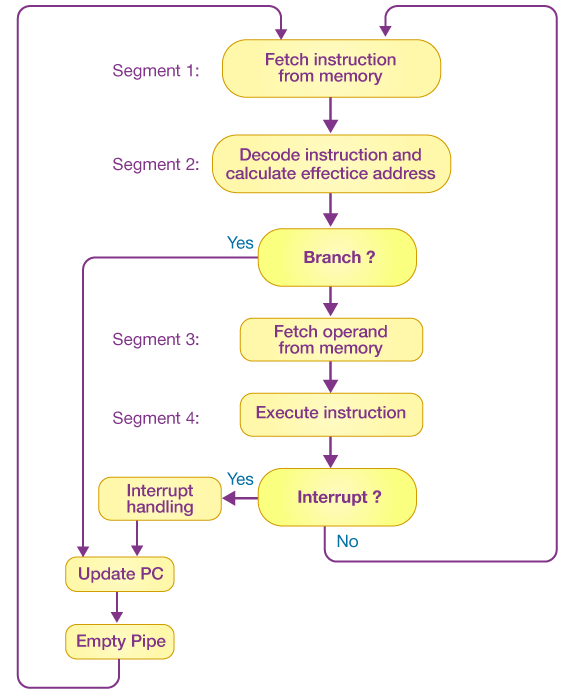
\includegraphics[scale=0.5]{./images/instruction-execution.png}
        \end{figure}

    \item To read from memory following steps are used.
    \begin{enumerate}
        \item Load MAR with address of memory where data is stored
        \item Initiate Memory Read operation.
        \item This will load MDR with the contents of memory.
    \end{enumerate}

    \begin{minipage}{\linewidth}
    \item Formulas
    \begin{myTableStyle} \begin{tabular}{ |m{6cm}|m{3cm}|m{5cm}| } \hline
        Stages                      &  k                & \\ \hline
        instructions                &  n                & \\ \hline
        Cycle Time                  &  \(T_c\)          &  Max(StageDelay) + Buffer Delay\\ \hline
        Total Time(Non-Pipeline)    &  \(T_{np}\)       &  \\ \hline
        Total Cycles(Pipeline)      &  k + (n-1)        & \(Time = P_c * T_c\) \\ \hline
        Total Cycles(Non-Pipeline)  &  n*k              & \(Time = (NP)_c * T_c\) \\ \hline
        Speed-up                    &  n*k/(k + (n-1))  & = k, n \(\gg\) k. \\ \hline
        Speed-up                    &   \( \boldsymbol { T_{np}\)/\(T_c } \)  &  \\ \hline
        Total Cycles(Pipeline, bubbles)&  k + (n-1) + b  & b = total bubbles \\ \hline
        Total Cycles(Pipeline, extra cycles)&  k + (n-1) + c  & c = extra cycles \\ \hline
        Average instrction execution time &  1 cycle + BPI & BPI=bubbles\_per\_instruction  \\ \hline
    \end{tabular} \end{myTableStyle} \vspace{0.08in}

    \item Time = T \quad No of Instructions = I \quad Cycles per instruction = CPI \quad Cycle Time = CT = 1/F
             \\ T = I x CPI x CT  \qquad  T = {\Large \( \frac{I * CPI}{F}  \) }

    \item Consider following instructions in a 5 stage pipeline. Number of cycles taken to execute without
           operator forwarding. Total stages(K)=5, Total instruction(n)=5
           \begin{myTableStyle} \begin{tabular}{ |m{2cm}|m{3cm}|m{2cm}|m{2cm}|m{3cm}| } \hline
              Instruction &         & Type      & Bubbles(b)& Cycles Taken  \\ \hline
              I1 &  R3 = R4 + R2    & R type    & 0         &   5(5+0) \\ \hline
              I2 &  R1 = M[addr]    & I type    & 0         &   1(1+0) \\ \hline
              I3 &  R1 = R2 + R3    & R type    & 2         &   3(1+2) \\ \hline
              I4 &  R4 = R1 + R3    & R type    & 2         &   3(1+2) \\ \hline
              I5 &  M[addr] = R4    & I type    & 2         &   3(1+2) \\ \hline
              Total Cycles &  k + (n-1) + b     & k=5, n=5  & b=6 &   15(5 + 4 + 6)\\ \hline
           \end{tabular} \end{myTableStyle} \vspace{0.08in}
    \end{minipage}

    \begin{minipage}{\linewidth}
    \item Consider following instructions in a 5 stage pipeline. Total stages(K)=5, Total instruction(n)=3
          Mutiplication takes 2, division takes 3 and addition takes 1 cycles in execution stage
           \begin{myTableStyle} \begin{tabular}{ |m{2cm}|m{3cm}|m{2cm}|m{3cm}|m{3cm}| } \hline
              Instruction &         & Type      & Extra Cycles(c)   & Cycles Taken  \\ \hline
              I1 &  R1 = R2 + R3    & R type    & 0                 &   5(5+0) \\ \hline
              I2 &  R4 = R5 * R6    & R type    & 1                 &   2(1+1) \\ \hline
              I3 &  R7 = R8 / R9    & R type    & 2                 &   3(1+2) \\ \hline
              Total Cycles &  k + (n-1) + c     & k=5, n=3  & c=3   &   10(5 + 2 + 3)\\ \hline
           \end{tabular} \end{myTableStyle} \vspace{0.08in}


    \item Consider a 4 stage pipeline processor.   The number of cycles needed by the four
             instructions I1, I2, I3, I4 in stages S1, S2, S3, S4 is shown below. What is the number of cycles needed to execute the loop - for(i=1 to 2) {I1; I2; I3; I4;}?

             \begin{myTableStyle} \begin{tabular}{ |m{1cm}|m{1cm}|m{1cm}|m{1cm}|m{1cm}| } \hline
                   & S1 & S2 & S3 & S4 \\ \hline
                I1 & 2  & 1  & 1  & 1  \\ \hline
                I2 & 1  & 3  & 2  & 2  \\ \hline
                I3 & 2  & 1  & 1  & 3  \\ \hline
                I4 & 1  & 2  & 2  & 2  \\ \hline
              \end{tabular} \end{myTableStyle} \vspace{0.08in}

    Hint : \quad S[ i ] [ j ] = max( top, left ) + stage\_time \\

   \begin{myTableStyle} \begin{tabular}{ |m{1cm}|m{1cm}|m{1cm}|m{1cm}|m{1cm}| } \hline
                   & S1 & S2 & S3  & S4 \\ \hline
                I1 & 2  & 3  & 4   & 5  \\ \hline
                I2 & 3  & 6  & 8   & 10  \\ \hline
                I3 & 5  & 7  & 9   & 13  \\ \hline
                I4 & 6  & 9  & 11  & 15  \\ \hline
                I1 & 8  & 10 & 12  & 16  \\ \hline
                I2 & 9  & 13 & 15  & 18  \\ \hline
                I3 & 11 & 14 & 16  & 21  \\ \hline
                I4 & 12 & 16 & 18  & 23  \\ \hline
              \end{tabular} \end{myTableStyle} \vspace{0.08in}

    \end{minipage}

    \begin{minipage}{\linewidth}
    \item Micro-operations
    \begin{enumerate}
        \item operations performed on data stored in registers are called Micro-operations.
        \item Micro-operations are predetermined for each instruction.
        \item Each instruction executes a sequence of pre-defined micro-operations.
        \item Common type of micro-operation : inter-register transfer, Arithmetic operations, Logic operations
              shift operation.
    \end{enumerate}
    \end{minipage}

    \item Important Registers : PC, MAR, MDR(MBR), AC, Named Registers(\(R_i\)), Pipeline Local Registers
    \item Add R1 [Mem] : R1 = R1 + [Mem] \\
    \begin{myTableStyle} \begin{tabular}{ |l|l|l|l|l| } \hline
        IF & \makecell[l]{ Instruction Decode \\ Read Operands \\from Mem and Reg}
        &execute & \makecell[l]{ MA \\ Load and \\Store}& WB   \\ \hline

        \makecell[l]{ MAR \(\leftarrow\) PC \\ Read Signal \\ Clear \large{ \( \boldsymbol R_y\)}  \\ Z \(\leftarrow\) PC + 1 }
        & \makecell[l]{ MAR \(\leftarrow\) IR[opr addr] \\ Read Signal } & Z \(\leftarrow\) MDR + \large{ \( \boldsymbol R_y\)}
        & & R1 \(\leftarrow\) Z \\ \hline

        \makecell[l]{ PC \(\leftarrow\) Z(Branch) \\ MDR is Loaded}
        & \makecell[l]{ \large{ \( \boldsymbol R_y\)} \(\leftarrow\) R1 \\ MDR is Loaded} & & & \\ \hline

        IR \(\leftarrow\) MDR & \makecell[l]{ Generate \\ Control Signals } & & & \\ \hline

    \end{tabular} \end{myTableStyle} \vspace{0.08in}

    \item  Control unit in a pipelined design.

    \item Instruction Cycle.\\
    \begin{myTableStyle} \begin{tabular}{ |l|m{6cm}|m{8cm}| } \hline
        IF & \makecell[l]{ 3 Steps and 4(6) micro-operation }
           & \makecell[l]{ (1) MAR \(\leftarrow\) PC, \quad Read Signal
                            \\ \; \; \; Clear {\large \( \boldsymbol R_y\)}, \quad Z \(\leftarrow\) PC + 1
                            \\ (2) PC \(\leftarrow\) Z(Branch), \quad MDR is Loaded
                            \\ (3)  IR \(\leftarrow\) MDR }  \\ \hline

        ID & Read operands from registers and Memory. Generate control signals.  Branch target is calculated
           & \makecell[l]{ (1) MAR \(\leftarrow\) IR[opr addr] \quad Read Signal
                          \\ (2) {\large \( \boldsymbol R_y\)} \(\leftarrow\) R1 \quad MDR is Loaded
                          \\ (3) Generate Control Signals} \\ \hline

        Exe & Performs ALU Oprn. Micro-operation sequence depends on opcode.
            & Z \(\leftarrow\) MDR + {\large \( \boldsymbol R_y\)}  \\ \hline

        MA & Load and Store instructions. Read or write the data memory. & \makecell[l]{ (1) LOAD : Z \(\leftarrow\) [Mem]
                                           \\ (2) STORE: [Mem] \(\leftarrow\) Z } \\ \hline

        WB & Write result in destination Register &  {\large \( \boldsymbol R_i\)}\(\leftarrow\) Z \\ \hline
    \end{tabular} \end{myTableStyle} \vspace{0.08in}

    \newpage

    \item IF Step
    \begin{enumerate}
        \item Put instruction in IR based on PC.
        \item Update PC to point to next instruction or branch.
    \end{enumerate}

    \item ID Step
    \begin{enumerate}
        \item For R-type instruction, read the operands(A, B) from the registers.
        \item For branch instruction, compute branch address(ALU\_Out)
    \end{enumerate}

    \item Execute Step
    \begin{enumerate}
        \item For R-type instruction, perform ALU operation. ALU\_Out = A {\large \(\oplus\)} B
        \item For branch instruction, (A==B)? \; PC=ALU\_Out
        \item For I-type instruction, compute memory reference(address, ALU\_Out).
    \end{enumerate}

    \item MA Step
    \begin{enumerate}
        \item For R-type instruction, set destination register(R = ALU\_Out). Check this.
        \item For I-type instruction, perform read/write operation on data memory.
        \item[WB-] For I-type instruction, set destination register(R = MDR)
    \end{enumerate}

    \item Structural Hazards.
    \begin{enumerate}
        \item Hardware resource conflicts among the instructions in the pipelin.
        \item Memory, a GPR Register, or an ALU
        \item Fetch cycle and Execution cycle both may need ALU at the same time. Fetching involves calculating Effective Address.
        \item multiple instruction in the pipe requires access to the very same resource in the same clock cycle.
        \item Solution: Introduce bubble
        \item Solution: Separate memory for Instruction and Data.
        \item Solution: Use of register files. Allows access to one write register, and one read register.
    \end{enumerate}

    \item Control Hazards
    \begin{enumerate}
        \item caused by branch instructions.
        \item Result of instruction determines the next instruction to be executed.
        \item Solution: Re-order instruction. The Compiler is used to implement this delayed branch.
        \item Solution: Introduce bubble(Stalling).
        \item Solution: Prediction.
        \item Solution: Dynamic Branch Prediction : Branch Table Buffer
        \item Solution: Delayed branching, a suitable instruction is placed below the conditional
              branch instruction which will be executed irrespective of whether branch is taken or
              not and won’t affect the program behavior.
        \item Branch penalty = total no of stalls.
        \item If the target address is present after the kth stage, then there will be (k – 1) stalls.
        \item Total number of stalls = Branch frequency * Branch Penalty
    \end{enumerate}

    \begin{minipage}{\linewidth}
    \item Data Hazards : RAW, WAR(anti dependency), WAW.
    \begin{enumerate}
        \item instruction is dependent on the results of a previous instruction.
        \item Bernstein condition.
        \item Solution: Re-order instruction by compiler.
        \item Solution: Introduce bubble or NOP instruction.
        \item Solution: Data forwarding sends data directly to the desired pipeline unit.
    \end{enumerate}

    \newpage

    \item Operand Forwarding(bipassing) for arithmetic instructions.
    \begin{enumerate}
        \item courses.cs.washington.edu/courses/cse378/07au/lectures/L12-Forwarding.pdf
        \item bypass the writeback and register read stages.
        \item for arithmetic instructions pass the ALU output without going through the register file.
        \item If there is a hazard, the operands will come directly from EX/MA or MA/WB pipeline registers.
        \item dependent instruction access registe's new value from the pipeline interface register directly.
        \item Operand Forwarding avoid stalls only if the dependent instructions are ALU type instructions.
        \item Without forwarding in 5 stage pipeline, we’d have to stall for two cycles.
        \item Hazards from R-type instructions can be avoided with forwarding.
    \end{enumerate}

    \begin{center}
    \begin{myTableStyle} \begin{tabular}{ c }
               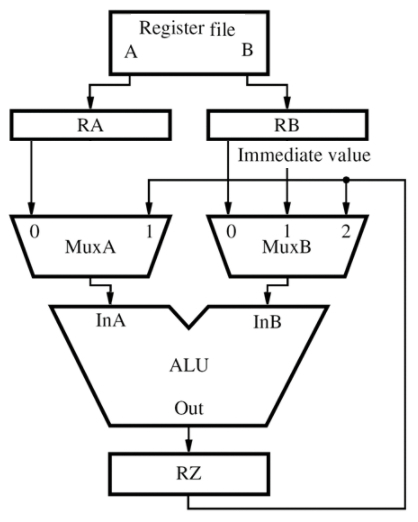
\includegraphics[scale=0.7]{./images/oprand_forwarding.jpeg}  \\
    \end{tabular} \end{myTableStyle} \vspace{0.08in}
    \end{center}
    \end{minipage}

    \newpage

    \item Operand forwarding(bipassing) for load instrctions.
    \begin{enumerate}
        \item When Load instruction is followed by instruction which uses load value as operand, then
              with operand forwarding pipeline gets stalled by 1 cycle.
        \item Loads can result in a "true" hazard, which must stall the pipeline.
        \item Load, store, branch and immediate instructions are I-type instructions.
        \item When all 3 operands are registers then instructions are R-type instructions.
        \item To-do : Determine number of stalls needed with and without operand forwarding.
    \end{enumerate}

    \item Register renaming, Branch Delay slot, reservation table and minimum average latency,
          anti dependency(WAR) between instructions

    \item Pipeline datapath \\
        \begin{figure}[h]
            \centering   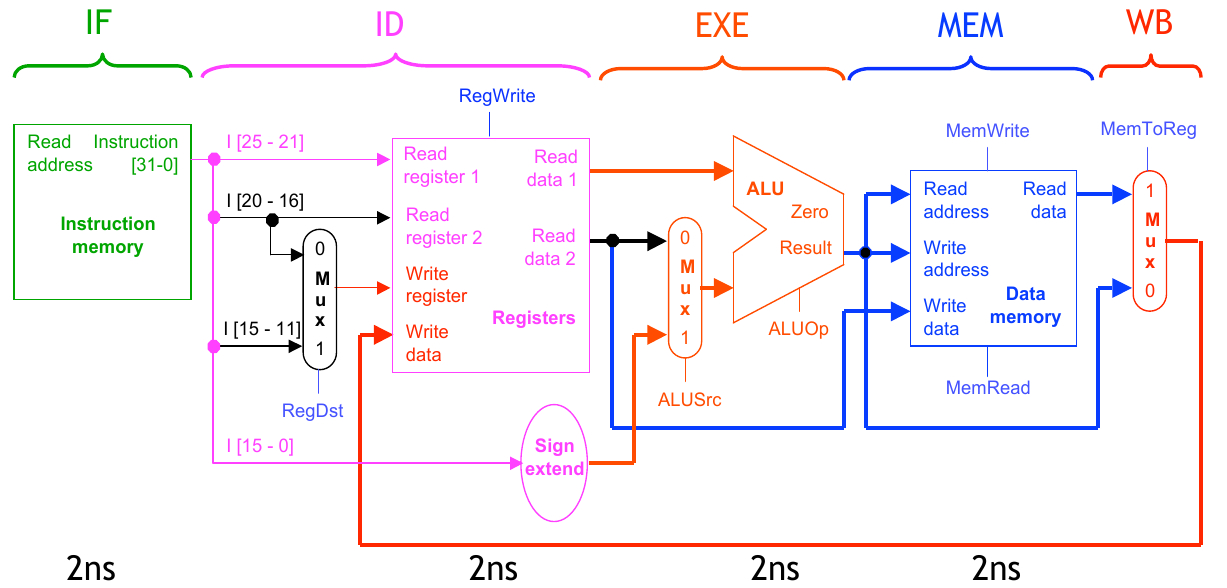
\includegraphics[scale=0.5]{./images/pipeline_datapath.jpeg}
        \end{figure}

\end{enumerate}
